\chapter{Background}
\label{sec:background}
This chapter provides an overview of the theoretical background of the methods used in this thesis. While the focus of this thesis is the application of machine learning methods in the quantum chemistry context, a basic introduction to compuatational quantum chemistry methods, namely self consistent field (SCF) methods, is provided. 

\section{Self Consistent Field (SCF) Theory}
\label{sec:background_scf}
Quantum chemistry has its roots far before the advent of the computer age. Based on the original theories on quantum mechanics formulated by Schrödinger and Heisenberg, the interest in the accurate description of matter via this new theory was sparked. After the introduction of the wave function by Schrödinger almost century ago Max Born's statistical interpretation enabled a direct calculation of the electrons density. \parencite{ref:schroedinger_1926undulatory} Already a year later Hartree coined a self consistant method to solve the many-electron problem utilizing a mean-field approach. Slater and Fock independently adapted the method by adding the exchange term and consistency with the Pauli exclusion principle. This method was later named Hartree-Fock (HF) method. \parencite{ref:Hartree_1928,ref:slater1930note,ref:fock1930naherungsmethode}. From that point on many advancements have been made in this field. Most prominently density functional therory (DFT), coupled cluster methods (CC), and perturbation theory (MP2) have been developed. Yet the theory behind the HF method is still the basis for many of these methods.

The following introductry overview of the Hartree-Fock method is largely based on the book by Szabo and Ostlund \parencite{ref:szabo_ostlund}. 

\subsection{Ideas behind the Hartree-Fock method}
\label{subsec:background_hf}
The Born Oppenheimer approximations allows the seperate treatment of the nuclear and electronic problem of a system. This is motivated by the vastly different masses and hence time-scales of nuclei and electrons. The total wavefunction of a system may be writen as a product state of electronic and nuclear wavefunction (using the convention of small letters for electrons and capital letters for nuclei coordinates):
\begin{equation}
    \Psi_{\text{tot}}(\mathbf{r}_n, \mathbf{R}_m) = \Psi_{\text{elec}}(\mathbf{r}_n; \mathbf{R}_m) \Psi_{\text{nuc}}(\mathbf{R}_m)
\end{equation}
Given our approximation the total wavefunction can be derived rather easily from the electronic wavefunction via an effective potential for the nuclear motion, given by a solved electronic wavefunction. However, we will focus on the prerequisit of the electronic wavefunction. It depends parametically on the nuclear coordinates and is the solution to the time independent Schrödinger equation:
\begin{equation}
    H_\text{elec} \Psi_{\text{elec}}(\mathbf{r}_n; \mathbf{R}_m) = E_{\text{elec}}(\mathbf{R}_m) \Psi_{\text{elec}}(\mathbf{r}_n; \mathbf{R}_m)
\end{equation}
With the electronic energy $E_{\text{elec}}$ being a functional of the electronic wavefunction which will be minimized under ceratin constraints as we'll see later. 
The Hamiltonian operator $H_\text{elec}$ reads: 
\begin{equation}
    H_\text{elec} = T + V_{\text{ne}} + V_{\text{ee}} = -\frac{1}{2} \sum_{i=1}^N \nabla_i^2 - \sum_{i=1}^N \sum_{A=1}^M \frac{Z_A}{|\mathbf{r}_i - \mathbf{R}_A|} + \sum_{i<j}^N \frac{1}{|\mathbf{r}_i - \mathbf{r}_j|}
\end{equation}
for $N$ electrons and $M$ nuclei in atomic units. 

%!Todo good start -> go on with Antisysmmetrization (part slater & fock introduced) - Hartree-Fock equations - .... - variational method + energy - matrices used - basis sets - SCF algorithm - kohn-sham equations & DFT - CC / other methods (short) - 
\section{Machine Learning}
\label{sec:background_ml}
%! Intor to ML & Statistical Learning. 
\subsection{Cost Functions}
\label{subsec:background_cost_function}
\TODO{also discuss f-score}

\section{QM9 dataset \parencite{ref:data_qm9}}
\label{sec:qm9}
During selection of a dataset for training two practical considerations dominate. 
\begin{enumerate}
    \item Cost per sample: Time savings through faster convergence are especially relevant for larger systems where the number of SCF iterations are and especially the number of integrals to be calculated are large. Stated differently, it is of very little interest to optimize guessing methods for small systems which converge nearly instantly on conventional hardware. 
    \item Fixed I/O size: Most ML models are constraint to a constant input and output size. 
\end{enumerate}
The QM9 dataset \parencite{ref:article1_qm9,ref:article2_qm9} ticks both of these two boxes. It offers a variety of molecules from as little as 3 constituent atoms up to 29 atoms. Additionally, there are large enough chunks of constitutional isomers to train models on these subsets of same sized matrices. The distribution of molecules by atom count with the predominant constitutional isomers is shown in \autoref{fig:method_qm9_overview}.
\begin{figure}[H]
    \centering
    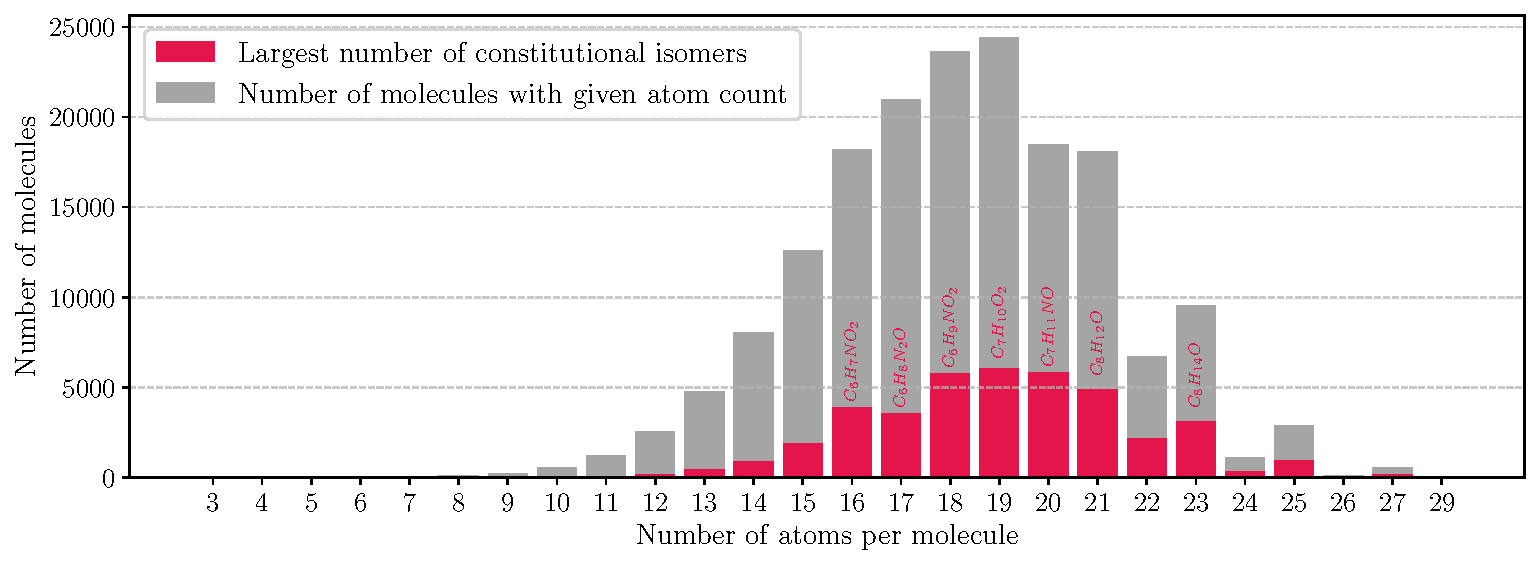
\includegraphics[width=\textwidth]{../fig/qm9_general/qm9_overview_stacked_bar.pdf}
    \caption[QM9 dataset overview]{Overview of the QM9 dataset. The dataset contains 134k molecules with up to nine heavy - \ch{C} \ch{O} \ch{N} \ch{F} - atoms. Large groups of constitutional isomers are present (largest depicted in red). The properties are calculated using DFT with the B3LYP functional and the 6-31G(2df,p) basis set.}
    \label{fig:method_qm9_overview}
\end{figure}
